% !TeX spellcheck = en_GB
% !TeX encoding = UTF-8

\section{Dictionary construction}
\label{sec:preproc:dict}
\index{dictionary construction}

\authorship{
  Portions of this section appear in the AFP entry \citetitle{hupel2017dict} (\citeauthor{hupel2017dict}~\cite{hupel2017dict}), and the preprint \citetitle{hupel2018dict} (\citeauthor{hupel2018dict}~\cite{hupel2018dict}).
  Users are recommended to refer to that AFP entry for latest documentation.
}

\noindent
Isabelle/Pure features \emph{type classes}~\cite{haftmann2007typeclasses,wenzel1997typeclasses}.
These are built into the kernel and are used extensively in theory developments.
The code generator, when targeting Standard ML, performs the well-known dictionary construction or \emph{dictionary translation}~\cite{haftmann2010codegeneration}.
This works by replacing type classes with records, instances with values, and occurrences with explicit parameters.

Similarly to Standard ML, CakeML does not support type classes.
To avoid complicating the correctness proofs, I decided to also not support them in the embedded term language (§\ref{sec:background:rewriting}).
Instead, a \emph{dictionary construction} eliminates classes and instances before embedding into the term language.
This section deals with the chosen encoding of type classes and instances, the certifying translation, and treatment of partial functions.

\subsection{Preliminaries}
\label{sec:preproc:dict:prelim}

\index{class parameter|see{class constant}}
\index{type class|see{class}}

In Isabelle parlance, the term \keyword{class} refers to a type class; a concept known from Haskell~\cite{wadler1989adhoc,haftmann2007typeclasses}.
A class can fix a type $\alpha$ and some constants whose type contains $\alpha$.
Those constants are officially referred to as \emph{class parameters}.
Classes and parameters live in different name spaces.
In the example in \cref{code:preproc:dict}, \holconst{plus} is a parameter of the \holconst{plus} class.
In this section, I will use the term \keyword{class constant} instead of class parameter, to avoid the ambiguity with function parameters.

A set of classes is called a \keyword{sort}.
Type variables may carry \emph{sort constraints}\index{sort constraint}, which are preceded by double colons: $\holtypejudgement{\alpha}{\{ \holclass{plus}, \holclass{times} \}}$.
Formally, a sort is an intersection of classes: the set of types that satisfy the sort $\{ \holclass{plus}, \holclass{times} \}$ is the set of the types have both a \holclass{plus} and a \holclass{times} \keyword{instance}.
Constants are said to have sort constrains if their types contain type variables with sort constraints.
Sort constraints can be omitted by the user and will be inferred.
If they are provided by the user, it is sufficient to specify them once per type variable.

As an example, consider the function $\holconst f\;x = x + x$.
In HOL, the $+$ operator is defined in the type class \holclass{plus}.
This means that the type of \holconst{f} is $(\holtypejudgement{\alpha}{\holclass{plus}}) \Rightarrow \alpha$.

Classes can extend other classes, with the inheritance relationship forming a directed acyclic graph (and with it, a partial order).
Sorts can be normalized according to this partial order.
Assuming that the class \holclass{group} extends both \holclass{zero} and \holclass{plus}, the sort $\{ \holclass{group}, \holclass{zero} \}$ can equivalently be written as $\{ \holclass{group} \}$.
I always assume that sorts are \emph{normal.}

Largely, classes work similarly in Haskell -- Haskell98, to be specific -- and Isabelle (see also §\ref{sec:preproc:dict:related}).
Isabelle's type system does not admit type constructor classes, nor other extensions like multi-parameter classes or undecidable instances.
However, Isabelle offers major enhancements over Haskell:
\begin{itemize}
  \item
    Isabelle being a proof assistant allows \emph{class axioms}\index{class axiom} that must be proved for every type that wishes to instantiate the class.
    The precise axioms are irrelevant for the dictionary construction (§\ref{sec:preproc:dict:elim:encoding}); they are abstracted as a predicate.
  \item
    It is possible to add edges in the inheritance relationship after the definition of the classes, as long as the user is able to produce a proof that the subclass axioms imply the superclass axioms.
\end{itemize}

\remark*{
  While parts of the dictionary construction are implemented incrementally, modifications in the class graph after their records have already been generated are not supported.
}

\subsection{Elimination of classes}
\label{sec:preproc:dict:elim}
The basic idea is to replace classes by \emph{dictionaries}\index{dictionary} containing all class constants and to replace instances by values.
Constants with sort constraints are rewritten in a way that they require additional dictionary parameters.

This transformation is an integral part of Isabelle's code generator.
It is described in detail by Haftmann and Nipkow \cite[§4]{haftmann2010codegeneration}, together with an informal correctness proof.

\begin{code}
  \begin{subfigure}{\linewidth}
    \begin{lstlisting}[language=Isabelle]
class plus =
  fixes plus :: $\alpha$ $\Rightarrow$ $\alpha$ $\Rightarrow$ $\alpha$ (infixl + 65)

definition f :: $\alpha$::plus $\Rightarrow$ $\alpha$ where
f //x// = //x// + //x//
    \end{lstlisting}
    \vskip-1.5em
    \caption{Source program}
  \end{subfigure}

  \vspace*{1em}
  \begin{subfigure}{\linewidth}
    \begin{lstlisting}[language=ML]
type 'a plus = {plus : 'a -> 'a -> 'a};
val plus = #plus : 'a plus -> 'a -> 'a -> 'a;

fun f dict x = plus dict x x;
    \end{lstlisting}
    \vskip-1.5em
    \caption{Target program (Standard ML)}
  \end{subfigure}
  \caption{Dictionary construction in Isabelle (current state)}
  \label{code:preproc:dict}
\end{code}

A complete example for $\holconst f\;x = x + x$ is reproduced in \cref{code:preproc:dict}.
Note that this translation is only required for target languages that do not support type classes (OCaml, Standard ML).
For other languages (Haskell, Scala), type classes are preserved with only minor syntactic changes.

\subsubsection{Current state}
\label{sec:preproc:dict:current}

In the code generator, the dictionary construction happens outside the logic.
It starts with a set of defining equations that represent the program to be exported.
These equations are proper theorems and are generated automatically by various commands for datatype and function definitions.
To improve efficiency, the user may provide alternative (verified) equations, for example, to replace a naive recursive implementation of a function by a more stack-efficient tail-recursive definition.

Then, these equations are internalized into an intermediate language.
The dictionary construction then proceeds in this internal language, following the approach outlined by Hall \etal~\cite{hall1996classes}.

\subsubsection{Certifying translation}
\label{sec:preproc:dict:elim:cert}

In this work, dictionary translation is performed before internalizing the defining equations into the deeply embedded term language.
It is a procedure implemented in ML which takes existing HOL definitions and produces new, derived HOL definitions, coupled with theorems certifying their equivalence.

\begin{code}
  \begin{lstlisting}[language=Isabelle]
datatype $\alpha$ dict_plus = mk_plus (const_plus: $\alpha$ $\Rightarrow$ $\alpha$ $\Rightarrow$ $\alpha$)

definition cert_plus :: $\alpha$::plus dict_plus $\Rightarrow$ bool where
cert_plus //dict// = (const_plus //dict// = plus)

fun f' :: $\alpha$ dict_plus $\Rightarrow$ $\alpha$ $\Rightarrow$ $\alpha$ where
f' //dict// //x// = const_plus //dict// //x// //x//

lemma f'_eq: cert_plus //dict// $\implies$ f' //dict// = f
(* proof omitted *)
  \end{lstlisting}
  \caption{Source program after dictionary construction in HOL (certifying translation)}
  \label{code:preproc:dict:hol}
\end{code}

To continue with the above example:
My mechanism introduces a derived constant \holconst{f'} with an additional dictionary parameter $\holtypejudgement{\mathit{dict}}{\alpha\;\holtype{dict\_plus}}$.
Then, it proves a theorem stating that for any \emph{valid} dictionary $\mathit{dict}$, \holconst{f'} is equivalent to \holconst{f}:
\[ \holconst{cert\_plus}\;\mathit{dict} \implies \holconst{f'}\;\mathit{dict} = \holconst{f} \]
Validity of a dictionary is captured by the $\holconst{cert\_plus}$ predicate.
Intuitively, $\holconst{cert\_}c\;\mathit{dict}$ means that $\mathit{dict}$ represents a known and lawful instance of class $c$.
The precise notion of ``validity'' is mainly dictated by technical considerations and discussed in the following section.

Additionally, for each type class instance $\holtypejudgement{\kappa}{(s_1, \ldots, s_k)\;c}$, where $\kappa$ is an $k$-ary type constructor and $s_i = \{c_{i,1}, \ldots, c_{i,n_i}\}$ are sorts, a new constant $\holconst{inst\_}c\holconst{\_}\kappa$ is defined.
Given the dictionaries for the $s_i$, it computes the dictionary for $\holtypejudgement{\kappa}{c}$.
Its correctness theorem is of the form
\[
  \left(\bigwedge\limits_{i=1}^{k} \bigwedge\limits_{j=1}^{n_i} \holconst{cert\_}c_{i,j}\;\mathit{dict}_{1,1}\right) \implies \holconst{cert\_}c\;(\holconst{inst\_}c\holconst{\_}\kappa\;\mathit{dict}_{1,1}\;\ldots\;\mathit{dict}_{1,n_1}\;\ldots\;\mathit{dict}_{k,1}\;\ldots\;\mathit{dict}_{k,n_k})
\]

\noindent For both instances and constants, each constituent class of each type variable's sort constraints gets assigned a dictionary argument and a premise certifying its validity.

The resulting program (as it would have been written by a user) is reproduced in \cref{code:preproc:dict:hol}.
My procedure defines the types and constants through the ML interfaces of various Isabelle packages, that is, users never see its results directly.
Instead, users would write \lstinline~declassify f~, which is a command that has the same effect as the hand-written definitions in \cref{code:preproc:dict:hol}.

\subsubsection{Possible encodings}
\label{sec:preproc:dict:elim:encoding}

The choice of the representation of dictionaries is straightforward:
I can model it as a datatype, along with functions returning values of that type.
The alternative here would have been to use Isabelle's extensible records \cite{naraschewski1998record}.
The obvious advantage of records is that I could easily model subclass relationships through record inheritance.
However, records do not support multiple inheritance.
Consequently, records offer no advantage over datatypes.
Instead, I opted for the more modern \holcommand{datatype} command \cite{blanchette2014datatypes}.
As of Isabelle2018, I have also introduced a \holcommand{datatype\_record} command that provides a subset of the syntax of records, but internally constructs a datatype.%
\thyrefdist{HOL-Library}{Datatype_Records}

A more controversial design question is how to represent dictionary certificates.
For example, given a value of type $\holtype{nat}\;\holtype{dict\_plus}$, how can one know that this is a faithful representation of the \holclass{plus} instance for \holtype{nat}?

\begin{enumerate}
  \item
    Florian Haftmann, in private communication, proposed a shallow encoding.
    It works by exploiting the internal treatment of constants with sort constraints in the Isabelle kernel.
    Constants themselves do not carry sort constraints, only their defining equations.
    The fact that a constant only appears with these constraints on the surface of the system is a feature of type inference.

    Instead, I can instruct the system to ignore these constraints.
    Isabelle's logic supports definitions of \emph{subtypes:}
    a type copy of an existing type that imposes additional constraints on values.
    For example, non-empty lists can be defined as a copy of lists with the constraint $\mathit{xs} \neq []$.
    Because HOL is a total logic, i.e., all types are non-empty, the system demands a witness satisfying the constraint.

    Applied to this situation, the key idea is to introduce a new type with a parameter $\alpha$ and the constraint that $\alpha$ implements a type class.
    However, this is ultimately futile:
    The nonemptiness proof requires a witness of a valid dictionary for an arbitrary, but fixed type $\alpha$, which is of course not possible, because type classes in general cannot be instantiated for all types.%
    \thyrefafp{Dict_Construction}{Impossibility}
  \item
    The certificates contain the class axioms directly.
    For example, the \holclass{semigroup\_add} class requires $(a + b) + c = a + (b + c)$.
    Such certificates are already defined for each class by Isabelle.
    Transferred to this setting, they would like this:
    %
    \begin{lstlisting}[language=Isabelle]
definition cert_plus :: $\alpha$ dict_plus $\Rightarrow$ bool where
cert_plus //dict// = ($\forall$//x// //y// //z//. const_plus //dict// (const_plus //dict// //x// //y//) //z// =
                               const_plus //dict// //x// (const_plus //dict// //y// //z//))\end{lstlisting}
    %
    Proving that instances satisfy this certificate is trivial.
    However, the equality proof of a constant before and after the construction is impossible: they are simply not equal in general.
    Nothing would prevent someone from defining an alternative dictionary using multiplication instead of addition and the certificate would still hold; but obviously functions using \holconst{plus} on numbers would expect addition.
    Intuitively, this makes sense: the above notion of certificate establishes no connection between original instantiation and newly generated dictionaries.

    Instead of proving equality, one would need to lift all existing theorems over the old constants to the new constants.
    This requires proof terms and replaying all proofs accordingly, which would be prohibitively expensive.
  \item
    In order for equality between new and old constants to hold, the certificate needs to capture that the dictionary corresponds exactly to the class constants.
    This is achieved by the representation in \cref{code:preproc:dict:hol}.
    It literally states that the fields of the dictionary are equal to the class constants.
    The condition of the resulting equation can only be instantiated with dictionaries corresponding to existing class instances.
    This constitutes a \emph{closed world} assumption, i.e., callers of generated code may not invent own instantiations.
\end{enumerate}

\noindent
My choice of representation is the third of these possibilities:
I expect dictionaries to be identical to the class constants.
For the user, that means that the conditions of the equivalence theorems ($\holconst{f'}\;\mathit{dict} = \holconst{f}$) can only be instantiated with existing class instantiations.
Unconditional equivalences can be achieved by monomorphizing constants.
Applied to the example in \cref{code:preproc:dict}, that would mean defining a constant $\holtypejudgement{\holconst{f}_\holtype{nat}}{\holtype{nat} \Rightarrow \holtype{nat}}$.
Its correctness theorem is unconditional, because no sort constraints occur in the type of \holconst{f}.

\subsection{Implementation}
\label{sec:preproc:dict:elim:impl}

The mechanism that transforms defining equations is similar to the one described by Haftmann and Nipkow~\cite[\S 4]{haftmann2010codegeneration}, which is presently used by the code generator to target OCaml and Standard ML.

\begin{figure}[t]
  \begin{subfigure}{.49\linewidth}
    \begin{lstlisting}[language=Isabelle]
class plus =
  fixes plus :: $\alpha$ $\Rightarrow$ $\alpha$ $\Rightarrow$ $\alpha$

instantiation nat :: plus
begin

fun plus_nat where
$0$ + //n// = (//n//::nat)
Suc //m// + //n// = Suc (//m// + //n//)

instance ..

end

definition f :: $\alpha$::plus $\Rightarrow$ $\alpha$ where
f //x// = //x// + //x//

(* f specialized to nat *)
definition g :: nat $\Rightarrow$ nat where
g //x// = f //x//
    \end{lstlisting}
  \end{subfigure}
  \begin{subfigure}{.49\linewidth}
    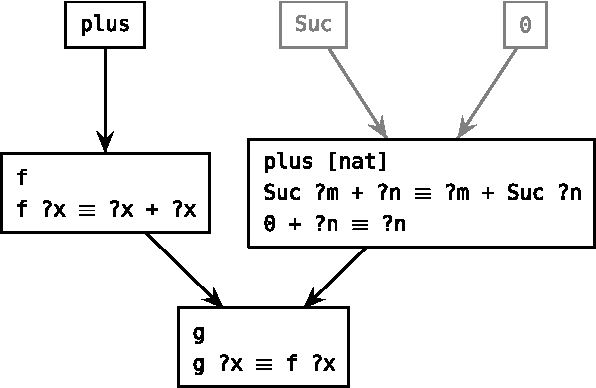
\includegraphics[width=\linewidth]{img/code-deps.pdf}
  \end{subfigure}
  \caption[A slightly extended source program and its code graph]{A slightly extended (from \cref{code:preproc:dict}) source program and its code graph}
  \label{fig:preproc:graph}
\end{figure}

Translating constants is the top-level operation in the dictionary construction.
The user invokes it with a set of constants.
Internally, the procedure uses existing mechanisms in Isabelle to obtain the \emph{code graph} of that set.
That graph contains all defining equations of the set and of all its transitive dependencies (i.e., other constants).
Each of these dependencies has to be re-defined as a new constant in some way, depending on whether or not it is a class constant.

\remark*{
  Strictly speaking, data constructors are also constants that may have class constraints.
  The dictionary construction does not support those in general.
  Additionally, the underlying type definition based on bounded natural functors largely ignores sort constraints.\footnote{\url{https://lists.cam.ac.uk/pipermail/cl-isabelle-users/2018-May/msg00065.html}}
  Consequently, they do not participate in the dictionary construction and are not relevant for this section.
}

\noindent
Along the way, auxiliary objects must be defined, for example the dictionary types for classes.
Unlike with the existing code generator, all of these steps need to be carried out inside the logic and are hence bound by its constraints.
Most notably, all definitions must be sequentialized to avoid forward references.
This means the implementation comprises mutually recursive, state-updating functions.

The code graph of a small program is given in \cref{fig:preproc:graph}.
As can be seen, the constant \holconst{g} depends on the constant \holconst{f} and the instance \holtypejudgement{\holtype{nat}}{\holclass{plus}}.
The data constructors \holconst{Suc} and \holconst{0} are greyed out.
The graph has to be traversed in topological order.

\remark*{
  Readers familiar with Isabelle's internals will notice that the code graph has been slightly redacted: The zero constructor for \holtype{nat} is actually the overloaded constant \holconst{zero} from the type class \holconst{zero}.
  This introduces technical complications, but does not in principle affect the dictionary construction.
}

\noindent
Throughout this section, the overloaded notations $\dict{\cdot}$ and $\dictinst{\cdot}$ are used to describe the translation of various kinds of objects.
I will first explain how types and classes themselves are processed.
Then, assuming a translation for terms exists, I will give a translation for type schemes and constants.
Lastly, the knot is tied by explaining how terms are processed.
In the actual implementation, all of these steps are intertwined.

\subsubsection{Types}

Recall that Isabelle distinguishes between type variables and schematic type variables\index{schematic variable} (§\ref{sec:background:types}).
Simple types, i.e., types that contain no schematic type variables, can be translated very easily: $\dict{\tau}$ forgets all sort constraints.
This is possible because those cannot have intrinsic sort constraints; those are imposed from the context and will be introduced accordingly when dealing with type schemes, which will be explained later.

\begin{code}[t]
  \begin{lstlisting}
datatype $\alpha$ dict_//c// = mk_//c//
  (super_$c_1$: $\alpha$ dict_$c_1$) (super_$c_2$: $\alpha$ dict_$c_2$) $\ldots$ (super_$c_n$: $\alpha$ dict_$c_n$)
  (const_$f_1$: $\dict{\tau_1}$) (const_$f_2$: $\dict{\tau_2}$) $\ldots$ (const_$f_m$: $\dict{\tau_m}$)

definition cert_//c// :: $\alpha$:://c// dict_//c// $\Rightarrow$ bool where
cert_//c// //dict// =
  (cert_$c_1$ (super_$c_1$ //dict//) $\wedge$ cert_$c_2$ (super_$c_2$ //dict//) $\wedge$ $\ldots$ cert_$c_n$ (super_$c_n$ //dict//) $\wedge$
   const_$f_1$ //dict// = $f_1$ $\wedge$ const_$f_2$ //dict// = $f_2$ $\wedge$ $\ldots$ $\wedge$ const_$f_m$ //dict// = $f_m$)
  \end{lstlisting}
  \caption{Dictionary datatype and certificate predicate}
  \label{code:datatype-cert}
\end{code}

\subsubsection{Classes}

A class $c$ over a type variable $\alpha$ may have superclasses $c_1, c_2, \ldots, c_n$ and constants $\holtypejudgement{f_1}{\tau_1}, \ldots, \holtypejudgement{f_m}{\tau_m}$.
Assuming the set $\{ c_1, c_2, \ldots, c_n\}$ is normal, this generates the definitions in \cref{code:datatype-cert}.
Note that the only type variable that may occur in the $\tau_i$ is $\alpha$ itself, which is an Isabelle restriction.
Consequently, it is not necessary to perform a recursive dictionary translation on the class constants, and I can get away with using the translation for simple types.

This newly introduced constructor and its fields have the following types:
\begin{align*}
  \holconst{mk\_}c &\holdoublecolon \alpha\;\holconst{dict\_}c_1 \Rightarrow \ldots \Rightarrow \alpha\;\holconst{dict\_}c_n \Rightarrow \alpha\;\holconst{dict\_}c \\
  \holconst{const\_}f_i &\holdoublecolon \alpha\;\holconst{dict\_}c \Rightarrow \dict{\tau_i} \\
  \holconst{super\_}c_i &\holdoublecolon \alpha\;\holconst{dict\_}c \Rightarrow \alpha\;\holconst{dict\_}c_i \\
  \holconst{cert\_}c &\holdoublecolon \holtypejudgement{\alpha}{c} \Rightarrow \holtype{bool}
\end{align*}
Apart from the certificate definition (which is only required for the correctness proofs), no sort constraints are left.

For any class constant $f$ of a class $\holconst{c}$, let \dictinst{f} denote the corresponding constant field.
If $d$ is a direct superclass of $c$, I use $\dictinst{c \leadsto d}$ to denote the corresponding superclass field.
In other words, $\dictinst{f} = \holtype{c}.\holconst{const\_}f$ and $\dictinst{c \leadsto d} = \holtype{c}.\holconst{super\_}d$.%

\begin{figure}[t]
  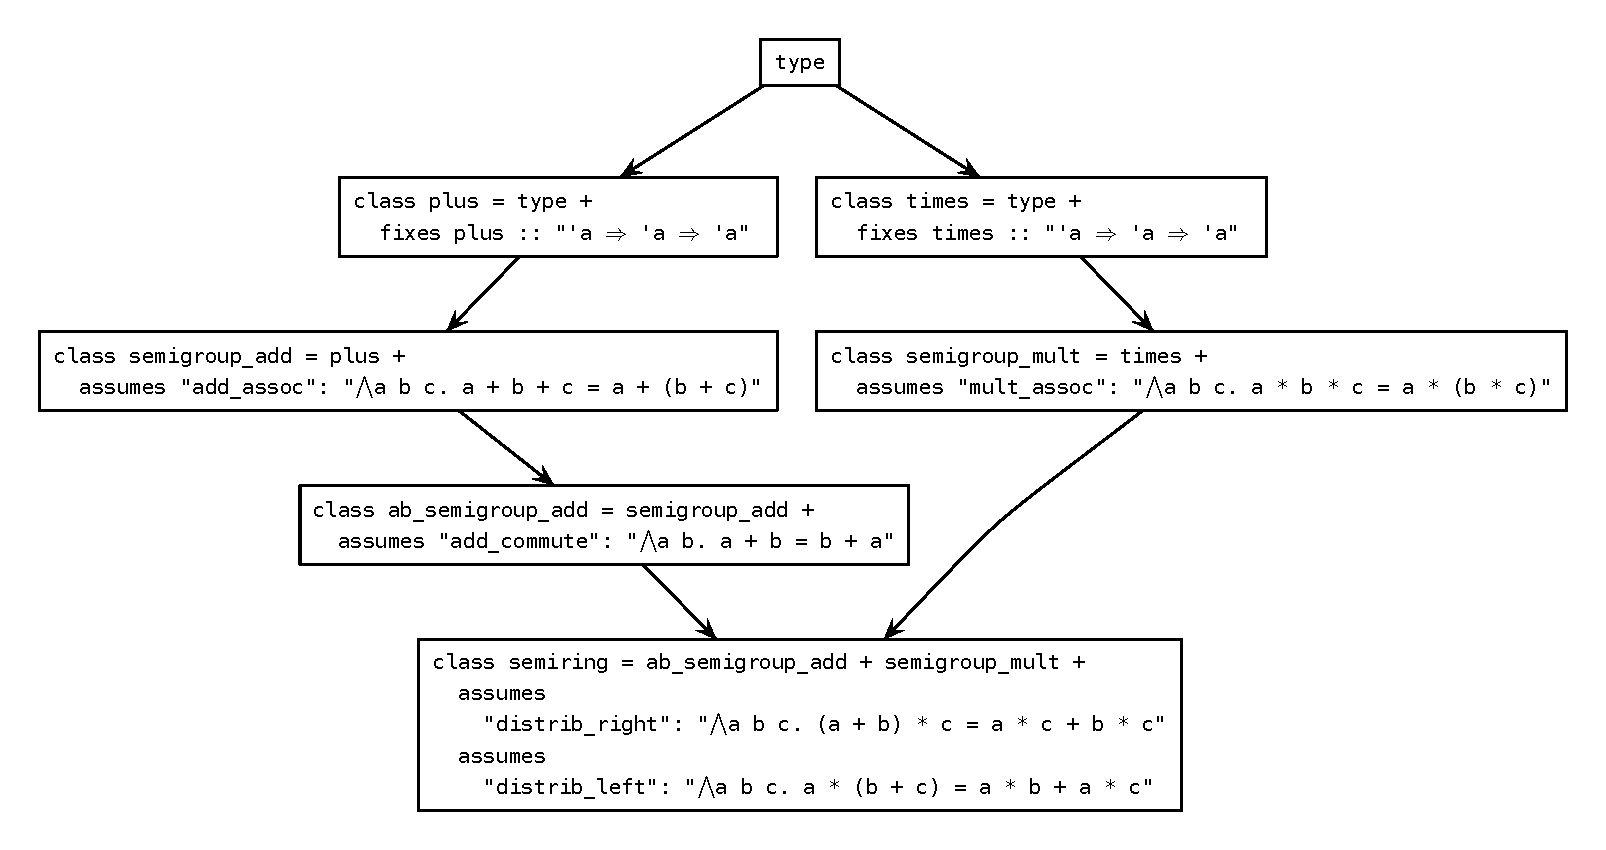
\includegraphics[width=\linewidth]{img/class-deps.pdf}
  \caption{Class hierarchy for the \holclass{comm\_semigroup\_add} class}
  \label{fig:preproc:hierarchy}
\end{figure}

\subsubsection{Superclass paths}

The class hierarchy in HOL is rather complex.
An excerpt, relating to the running example, is reproduced in \cref{fig:preproc:hierarchy}.
For example, to obtain the \holconst{plus} operation from a \holclass{semiring} constraint, one has to follow three subclass--superclasses edges.

In general, for any two classes $c$ and $d$, there may be multiple different paths from the subclass $c$ and the (possibly indirect) superclass $d$.
It is not obvious that the choice of path is irrelevant for the semantics of the generated program, i.e., that the system is \emph{coherent} according to Jones~\cite{jones1994types}. Isabelle's type system guarantees coherence \cite{nipkow1991typeclasses,nipkow1995reconstruction}, which the dictionary construction assumes.
If that assumption were violated, the equivalence proof (§\ref{sec:preproc:dict:equiv}) would fail.
Coherence is consequently a meta-theorem and not internalised in the logic.

For the purpose of this presentation, it is sufficient to assume that the implementation uses the ``first'' path according to the kernel-defined order of superclasses.
It is straightforward to extend the notation $\holtypejudgement{\dictinst{c \leadsto d}}{\alpha\;\holconst{dict\_}c \Rightarrow \alpha\;\holconst{dict\_}d}$ for an indirect superclass $d$ of $c$, where the edges are conjoined using the function composition operator $\circ$.

\subsubsection{Non-class constants}

Class constants can be easily distinguished from non-class ones:
The former have no defining equations.
They are only given meaning by an instance of a class.

In the example in \cref{fig:preproc:graph}, the constants \holconst{f}, \holconst{g} and \holconst{plus\_nat} are non-class constants, whereas \holconst{plus} is a class constant.
This is reflected in the graph: the box for \holconst{plus} has no defining equations.
Note that while \holconst{plus\_nat} participates in the instantiation of a type class, it is itself not considered to be a class constant.

Assume a transformation of a non-class constant $f$ with a set of defining equations $\mathit{eq}_i$.
Each of the $\mathit{eq}_i$ is of the form $f\;p_{i,1}\;p_{i,2}\;\ldots\;p_{i,n_i} \equiv \mathit{rhs}_i$, with the $p_{i,j}$ being constructor patterns.
Furthermore, the type of $f$ is a type scheme, i.e., it is of the form $\forall \holtypejudgement{\alpha_1}{s_1} \ldots \forall \holtypejudgement{\alpha_k}{s_k}.\; \tau$.
Each of the schematic type variables $\alpha_i$ may carry a sort constraint $s_i = \{ c_{i,1}, \ldots, c_{i,m_i} \}$ that is assumed to be normal.

Let $\dict{t}_\Gamma$ denote the translation of terms in a context $\Gamma$ (to be defined later).
Also, let \dictinst{f} mean a fresh name, e.g.\ $f'$ to refer to the newly defined constant.

I can now explain the translation of the defining equations.
Each equation $\mathit{eq}_i$ gives rise to a new equation $\dict{\mathit{eq}_i}$ as follows:
\begin{itemize}
  \item For every class constraint of every type variable, a new parameter is introduced.
  \item The existing parameters stay unchanged, because data constructors do not participate in the dictionary construction.
  \item The right-hand side is translated with all new parameters as context.
\end{itemize}

\noindent
Formally:
\begin{align*}
  \dict{\mathit{eq}_i} &= (\mathit{lhs}'_i \equiv \dict{\mathit{rhs}_i}_\Gamma) \\
  \Gamma &= [ \mathit{dict}\_c_{1,1}, \ldots, \mathit{dict}\_c_{k,m_k} ] \\
  \mathit{lhs}'_i &= \dictinst{f}\;(\holtypejudgement{\mathit{dict}\_c_{1,1}}{\alpha_1\;\holconst{dict}\_c_{1,1}})\;\ldots\;(\holtypejudgement{\mathit{dict}\_c_{k,m_k}}{\alpha_k\;\holconst{dict}\_c_{k,m_k}})\;p_{i,1}\;p_{i,2}\;\ldots\;p_{i,n_i}
\end{align*}

\noindent
Note that the translation for left-hand and right-hand sides differs:
left-hand sides, consisting only of patterns, need no context.

All resulting equations are considered as defining equations for \dictinst{f}.
Subsequently, they are fed into the internal interface of the \holcommand{function} command to produce a new logical constant.
The additional technical challenges of this are documented in the following sections.

\subsubsection{Instance definitions and composition}

An instance $\holtypejudgement{\kappa}{(s_1, \ldots, s_k)\;c}$ is treated as if it is a (non-class) constant with no arguments, returning a dictionary containing instantiations of all class constants.
Consequently, each instance gives rise to a new definition that I refer to as $\dictinst{\holtypejudgement{\kappa}{c}}$.

However, it is also necessary to compose instances from contexts.
This might mean a combination of following along superclass paths and applying instance definitions to arguments.
I use $\dict{\holtypejudgement{\tau}{c}}_\Gamma$ as notation for this, where $\tau$ is a simple type and $\Gamma$ a context.

I will first describe the (deterministic) algorithm to obtain $\dict{\holtypejudgement{\tau}{c}}_\Gamma$.
\begin{enumerate}
  \item
    If $\tau$ is a type variable, find an instance $\mathit{dict}$ for $\holtypejudgement{\tau}{c'}$  in $\Gamma$ where $c'$ is a subclass of $c$.
    Then, $\dict{\holtypejudgement{\tau}{c}}_\Gamma = \dictinst{c' \leadsto c}\;\mathit{dict}$.
  \item
    Otherwise, $\tau$ is of the form $(\tau_1, \ldots, \tau_k)\;\kappa$, i.e., a $k$-ary type constructor $\kappa$ applied to $k$ types.
    Find an instance definition $\holtypejudgement{\kappa}{(s_1, \ldots, s_k)\;c'}$ where:
    \begin{itemize}
      \item $c'$ is a subclass of $c$ and
      \item for each constraint $\holtypejudgement{\tau_i}{c_{i,j}}$ stemming from the $s_i$, $r_{i,j} = \dict{\holtypejudgement{\tau_i}{c_{i,j}}}_\Gamma$ is defined
    \end{itemize}
    Then, $\dict{\holtypejudgement{\tau}{c}}_\Gamma = \dictinst{c' \leadsto c}\;(\dictinst{\holtypejudgement{\kappa}{c'}}\;r_{1,1}\;\ldots\;r_{k,m_k})$.
  \item
    If no suitable instance exists, fail.
\end{enumerate}

\noindent For any well-sorted judgement $\holtypejudgement{\tau}{c}$, this algorithm is guaranteed to find at least one composed instance.
Similar to finding superclass paths, the choice of instance is irrelevant.
This is a meta-theorem based on the \emph{coregularity} property that is guaranteed by Isabelle's type system \cite{nipkow1991typeclasses,nipkow1995reconstruction}.

It remains to treat instance definitions $\dictinst{\holtypejudgement{\kappa}{c}}$.
Assuming the same naming conventions as above, the generated definition is of the following form:
\[
  \dictinst{\holtypejudgement{\kappa}{c}}\;\mathit{dict}_{1,1}\;\ldots = \holconst{mk\_}c\;\dict{\holtypejudgement{(\alpha_1, \ldots, \alpha_k)\;\kappa}{c_1}}_\Gamma\;\ldots\;\;\dict{\holtypejudgement{(\alpha_1, \ldots, \alpha_k)\;\kappa}{c_n}}_\Gamma\;\dict{f_1}_\Gamma\;\ldots\;\dict{f_m}_\Gamma
\]

\subsubsection{Terms}

I define the translation of terms \dict{t} that are not constants recursively as follows:
\begin{align*}
  \dict{x}_\Gamma &= x &\text{(where $x$ is a variable)} \\
  \dict{t\;u}_\Gamma &= \dict{t}_\Gamma\;\dict{u}_\Gamma \\
  \dict{\lambda x.\,t}_\Gamma &= \lambda x.\,\dict{t}_\Gamma
\end{align*}
The rule for constants is a bit more involved.
Let $f$ be a constant with $k$ type parameters, i.e., of type scheme $\forall \holtypejudgement{\alpha_1}{s_1} \ldots \forall \holtypejudgement{\alpha_k}{s_k}$.
In any occurrence of $f$ in a term, these type parameters are instantiated with simple types $\tau_1, \ldots, \tau_k$.
\[
  \dict{f}_\Gamma = \dictinst{f}\;\dict{\holtypejudgement{\tau_1}{c_{1,1}}}_\Gamma\;\ldots\;\dict{\holtypejudgement{\tau_k}{c_{k,m_k}}}_\Gamma
\]

\subsubsection{Challenges}

In the standard case, where the user has not performed a custom code setup, the resulting function looks similar to its original definition.
But the user may have also changed the implementation of a function significantly afterwards.
This poses some challenges:

\begin{itemize}
  \item
    The new constants need to be proven terminating.
    The routine heuristically transfers the original termination proof to the new definitions (§\ref{sec:preproc:dict:termination}).
    This only works when the termination condition does not rely on class axioms.
  \item
    The domain of functions must be tracked, because even though HOL is a total logic, functions may be under-specified.
    Congruence rules are used to construct an inductive predicate (§\ref{sec:background:inductive}) representing the \emph{side condition} of a function (§\ref{sec:preproc:dict:partial}).
  \item
    In order to fine-tune executable code, the code generator allows users to specify different constructors of a datatype than those it has been defined with, or even to introduce constructors for non-datatypes.
    However, the \holcommand{function} command does not support that in general (§\ref{sec:preproc:limitations}).
    But even if it did, the equivalence of old and new definition may become conditional on invariants, which is conceptually not supported (§\ref{sec:preproc:limitations}).
  \item
    The set of defining equations must be non-overlapping to ensure determinism.
    Additionally, to accommodate for later phases in the compiler (§\ref{sec:intermediate:elim}), some pattern variables need to be renamed (§\ref{sec:preproc:compatibility}).
\end{itemize}


\subsection{Preservation of termination}
\label{sec:preproc:dict:termination}

\begin{code}[t]
  \begin{lstlisting}
fun f :: nat $\Rightarrow$ nat where
f $0$ = $0$
f (Suc //n//) = f //n//

lemma [code]: f //x// = f //x// by simp\end{lstlisting}
  \caption{Pathological example of a non-terminating defining equation}
  \label{code:non-terminating}
\end{code}

As indicated above, the newly defined functions must be proven terminating.
In general, I cannot reuse the original termination proof, as the example in \cref{code:non-terminating} illustrates.
While the original function is primitively recursive, and hence trivially proved to be terminating, the user has added a defining equation that characterizes a non-terminating implementation.
My construction cannot deal with such pathological cases, but fortunately they are rare in practice.
The invocation of the dictionary construction would just fail for this example.

Instead, based on my experience, the most common cases are that users either
\begin{itemize}
  \item do not adapt the defining equations at all,
  \item adapt them without changing the termination scheme, or
  \item adapt them to use different recursive calls, while still being terminating.
\end{itemize}

\noindent
For the last case, it is impossible to port the existing termination proof, because it is not applicable any more.
Hence, the construction falls back to use the same automated proof method as the \holcommand{function} package.

However, the other cases are more interesting.
In the remainder of this section, I will illustrate the first case, which is a specialization of the second one.%
\thyrefafp{Dict_Construction}{Termination}
The original termination proof should intuitively be still applicable.

The running example will be a function that sums up values in a list.
%
\begin{lstlisting}
fun sum_list :: $\alpha$::{plus,zero} list $\Rightarrow$ $\alpha$ where
sum_list [] = //0//
sum_list (//x// # //xs//) = //x// + sum_list //xs//
\end{lstlisting}
%
This function carries two distinct class constraints -- arising from the use of addition and zero, both of which are provided by a class in Isabelle -- which are translated into two dictionary parameters:
%
\begin{lstlisting}[language=Isabelle]
sum_list' //dict_plus// //dict_zero// [] =
    const_zero //dict_zero//
sum_list' //dict_plus// //dict_zero// (//x// # //xs//) =
    const_plus //dict_plus// //x// (sum_list' //dict_plus// //dict_zero// //xs//)
\end{lstlisting}
%
Here, the termination argument has not changed:
While two additional parameters have been introduced, they remain unchanged in between recursive calls.
Observe that whenever sort constraints are present, the dictionary construction always introduces new arguments, but keeps the termination scheme.

Now, the termination of \holconst{sum\_list'} must be proved.
The \holcommand{function} package analyses the structure of recursive calls and collects them into a set of constraints.

As a notation for constraints, I will use $\bar{p} \leadsto \bar{x}$.
$\bar{p}$ stands for the (tupled) patterns on the left-hand side of an equation and $\bar{x}$ for the (also tupled) actual parameters passed to a recursive invocation.
Only variables bound in $\bar{p}$ may appear in $\bar{x}$.

\remark*{
  The \holcommand{function} command not only tracks the parameters passed to a recursive call, but also, under which conditions such a call appears.
  For example, a recursive call may appear in a \holkeyword{then} or \holkeyword{else} branch.
  To properly represent that, the notation needs to be extended to allow for arbitrary predicates.
  For explaining the termination heuristics, this generality is not needed; but it will be revisited for another purpose in §\ref{sec:preproc:dict:partial}.
}

\noindent
For the above example, this looks as follows:
%
\begin{align}
  \{ (x \cons \mathit{xs}) &\leadsto \mathit{xs} \} \tag{\holconst{sum\_list}} \\
  \{ (\mathit{dict\_plus}, \mathit{dict\_zero}, x \cons \mathit{xs}) &\leadsto (\mathit{dict\_plus}, \mathit{dict\_zero}, \mathit{xs})\} \tag{\holconst{sum\_list'}}
\end{align}
%
Internally, for every function $\holtypejudgement{f}{\sigma_1 \Rightarrow \sigma_2 \Rightarrow \ldots \Rightarrow \sigma_n \Rightarrow \tau}$, the package defines an inductive relation $\holtypejudgement{f\_\holconst{rel}}{(\sigma_1, \sigma_2, \ldots, \sigma_n) \Rightarrow (\sigma_1, \sigma_2, \ldots, \sigma_n) \Rightarrow \holtype{bool}}$ with one introduction rule per constraint.
Note that the arguments are tupled, i.e.\ all function arguments participate in the definition of this \emph{termination relation.}

In the example, the predicate \holconst{sum\_list\_rel} is defined by the following introduction rule:
\[
  \inferrule*{ }{
    \holconst{sum\_list\_rel}\;\mathit{xs}\;(x \cons \mathit{xs})
  }
\]

\noindent
For details on how the \holcommand{function} package assembles the termination relation based on the constraints, in particular for more complicated recursion schemes, refer to Krauss' thesis~\cite{krauss2009fun}.

To prove that a function terminates, it is sufficient to show that its termination relation is \emph{well-founded.}
In the majority of cases, this happens by supplying a suitable \emph{measure function} that maps the arguments to natural numbers and decreases for each recursive call.
The \holcommand{function} package is able to try out various measure functions automatically.

In this setting however, the termination of $f$ has already been proved, either automatically or by the user.
The construction tries to re-use that proof, i.e., the well-foundedness theorem of $f\_\holconst{rel}$, for the proof of well-foundedness of $f'\_\holconst{rel}$, where $f'$ is the result of applying the dictionary construction to $f$.
Except for the additional (unchanging) dictionary arguments, these relations are more or less equivalent to each other.

\begin{lemma}[Well-founded simulation]
  Let $\holtypejudgement{P}{\tau \Rightarrow \tau \Rightarrow \holtype{bool}}$ be a well-founded relation and $\holtypejudgement{g}{\sigma \Rightarrow \tau}$ a function such that
  \[
    \forall x\; y.\; P'\;x\;y \implies P\;(g\;x)\;(g\;y)
  \]
  Then, $\holtypejudgement{P'}{\sigma \Rightarrow \sigma \Rightarrow \holtype{bool}}$ is also a well-founded relation.
\end{lemma}

\begin{figure}[t]
  \centering
  \tikzstyle{r} = [circle, fill=gray!10, text width=1.5em, text height=1em, text centered, node distance=2cm]
  \tikzstyle{rprime} = [circle, fill=gray!30, text width=1.5em, text height=1em, text centered, node distance=2cm]
  \tikzstyle{simline} = [draw, -latex', densely dashed, thick]
  \tikzstyle{line} = [draw, -latex]

  \begin{tikzpicture}
    \node [r] (rx1) {$x_1$};
    \node [r, right of=rx1] (rx2) {$x_2$};
    \node [r, right of=rx2] (rx3) {$x_3$};
    \node [left of=rx1, node distance=2cm] {$P$};
    \node [right of=rx3, node distance=1.5cm] (rx4) {$\ldots$};

    \node [rprime, below of=rx1, node distance=3cm] (rpx1) {$x_1'$};
    \node [rprime, right of=rpx1] (rpx2) {$x_2'$};
    \node [rprime, right of=rpx2] (rpx3) {$x_3'$};
    \node [left of=rpx1, node distance=2cm] {$P'$};
    \node [right of=rpx3, node distance=1.5cm] (rpx4) {$\ldots$};

    \path [simline] (rpx1) -- (rx1) node [midway, right] {$g$};
    \path [simline] (rpx2) -- (rx2) node [midway, right] {$g$};
    \path [simline] (rpx3) -- (rx3) node [midway, right] {$g$};
    \path [line] (rx1) -- (rx2);
    \path [line] (rx2) -- (rx3);
    \path [line] (rx3) -- (rx4);
    \path [line] (rpx1) -- (rpx2);
    \path [line] (rpx2) -- (rpx3);
    \path [line] (rpx3) -- (rpx4);
  \end{tikzpicture}
  \caption{Well-founded simulation}
  \label{fig:preproc:dict:wfsim}
\end{figure}

\noindent
This theorem allows to \emph{simulate} the structure of the recursive calls of $f'$ with those of $f$ (depicted in \cref{fig:preproc:dict:wfsim}).
There is an important difference, though: $f\_\holconst{rel}$ may have sort constraints, $f'\_\holconst{rel}$ does not.

Instantiating the above lemma with the two termination relations entails choosing a suitable function $g$ that maps arguments of \holconst{sum\_list'} to arguments of \holconst{sum\_list}, i.e., a function of type
\[ (\alpha\;\holtype{dict\_plus} \times \alpha\;\holtype{dict\_zero} \times \alpha\;\holtype{list}) \Rightarrow (\holtypejudgement{\beta}{\{ \holclass{plus}, \holclass{zero} \}}) \;\holtype{list} \]
for an arbitrary type $\beta$.
Obviously, $g$ can drop the first two elements of the tuple.
The challenge arises when trying to map a list with element type $\alpha$ to one with element type $\beta$.
I cannot instantiate $\beta = \alpha$, because $\beta$ carries a sort constraint.

In a parametric setting, this would be the end of it, because it is impossible to write such a function~\cite{reynolds1983parametric,lochbihler2016probabilistic,gilcher2017parametricity}.
Isabelle however offers an escape hatch: recall that all types are non-empty.
The polymorphic constant $\holtypejudgement{\holconst{undefined}}{\alpha}$\holconstindex{undefined} can serve as a witness for an arbitrary type.
Assuming that there is at least one concrete type $\tau$ that satisfies the sort constraints of $\beta$, I can instantiate $\beta = \tau$.
The desired mapping function can now be specified as follows:
\[ g\;(\_, \_, \mathit{xs}) = \holconst{map}\;(\lambda \_.\;\holtypejudgement{\holconst{undefined}}{\tau})\;\mathit{xs} \]
In case there is no such concrete $\tau$, the above expressions fails to type check, causing the heuristic to fail.%

It remains to show how the premise of the well-founded simulation theorem is proved in this particular case:
\[
  \forall x\; y.\; \holconst{sum\_list'\_rel}\;x\;y \implies \holconst{sum\_list\_rel}\;(g\;x)\;(g\;y)
\]
The proof proceeds by induction using the induction principle of the \holconst{sum\_list'\_rel} inductive predicate, which gives one case per introduction rule, that is:
\[
  \forall \mathit{d\_plus}\;\mathit{d\_zero}\;x\;\mathit{xs}.\;\holconst{sum\_list\_rel}\;(g\;(\mathit{d\_plus}, \mathit{d\_zero}, \mathit{xs}))\;(g\;(\mathit{d\_plus}, \mathit{d\_zero}, x \cons \mathit{xs}))
\]
After unfolding the definition of $g$:
\[
  \forall \mathit{xs}.\;\holconst{sum\_list\_rel}\;(\holconst{map}\;(\lambda \_.\;\holconst{undefined})\;\mathit{xs})\;(\holconst{undefined}\cons \holconst{map}\;(\lambda \_.\;\holconst{undefined})\;\mathit{xs})
\]
This can now trivially be proved by using the introduction rule of \holconst{sum\_list\_rel}.

\remark*{
  This construction critically depends on the non-emptiness of types and that there is at least one type satisfying the sort constraints of a function.
  In that sense, it only works because HOL admits non-parametric definitions~\cite{reynolds1983parametric,lochbihler2016probabilistic,gilcher2017parametricity}.
}

\noindent
More generally, this construction allows the proof of well-foundedness of any relation
\[\holtypejudgement{R'}{(\beta_1 \times \ldots \times \beta_n \times (\alpha_1, \ldots, \alpha_k)\;\tau) \Rightarrow (\beta_1 \times \ldots \times \beta_n \times (\alpha_1, \ldots, \alpha_k)\;\tau) \Rightarrow \holtype{bool}}\]
given a well-founded relation
\[\holtypejudgement{R}{(\alpha_1, \ldots, \alpha_k)\;\tau' \Rightarrow (\alpha_1, \ldots, \alpha_k)\;\tau' \Rightarrow \holtype{bool}}
\]
where $\tau$ is a suitable type constructor equipped with a functorial $\holconst{map}_\tau$, $\tau$ and $\tau'$ differ only in sort constraints, $R$ and $R'$ are structurally equivalent and parametric in all $\alpha_i$.

\remark*{
  The precise nature of ``suitability'' is not relevant for the discussion.
  In the implementation, bounded natural functors as introduced by Blanchette~\etal~\cite{blanchette2017bnf,blanchette2014datatypes} without dead variables are considered suitable.
}

\noindent
The mapping function $g$ is defined as follows:
\begin{align*}
  &\holtypejudgement{g}{(\beta_1 \times \ldots \times \beta_n \times (\alpha_1, \ldots, \alpha_k)\;\tau) \Rightarrow (\alpha_1, \ldots, \alpha_k)\;\tau'} \\
  &g\;(\_, \ldots, \_, t) = \holconst{map}_\tau\;\underbrace{(\lambda \_.\; \holconst{undefined})\;\ldots\;(\lambda \_.\; \holconst{undefined})}_{\text{one for each $\alpha_i$}}\;t
\end{align*}

\subsection{Partially specified functions}
\label{sec:preproc:dict:partial}

HOL is a total logic, that is, it is always possible to assign a value to a function $\holtypejudgement{f}{\alpha \Rightarrow \beta}$ applied to any argument $\holtypejudgement{x}{\alpha}$.
This immediately raises the question how to represent \emph{partially specified} (or \emph{under-specified}) functions, e.g.\ to obtain the head of a list:
%
\begin{lstlisting}[language=Isabelle]
fun hd :: $\alpha$ list $\Rightarrow$ $\alpha$ where
hd (//x// # //xs//) = //x//
\end{lstlisting}
%
Obviously, in this function definition, the case for the empty list is omitted.
Note that under-specification and non-termination are different kinds of partiality; the latter of which is not supported by this work.

\remark*{
  It is possible to define and reason about non-terminating functions in Isabelle.
  However, both the dictionary construction and the deep embedding steps~(§\ref{sec:deep}) are unable to process such definitions.
  Other steps of the pipeline, in particular the verified part~(§\ref{sec:compiler}), do not presuppose termination of the original equations.
}

\noindent
There are various ways to deal with under-specification (a more detailed survey is given in §\ref{sec:preproc:dict:related}):

\begin{enumerate}
  \item
    Lift the result type into \holtype{option}, i.e.\ $\alpha \Rightarrow \beta$ turns into $\alpha \Rightarrow \beta\;\holtype{option}$.
    Arguments for which the function is not specified get assigned a \holconst{None} value.
    The domain of the function $\holconst{dom}_f$ can conveniently be expressed as a set $\{ x \mid f\;x \neq \holconst{None} \}$.
  \item
    Function definitions are ``artificially'' completed to be always specified.
    In HOL, \holconst{undefined} is an unspecified constant of arbitrary type.
    The meta-theorem about this unspecified constant is that for all predicates $P$, $P\;\holconst{undefined}$ is provable if and only if $P\;x$ is provable for all $x$.
  \item
    Based on the function equations, derive a set carrying the \emph{side condition} of the function and allow reasoning over a function application $f\;x$ only if $x \in \holconst{side}_f$ holds.
    This is comparable to refinement types \cite{gordon2010refinement}, but where the constraints are external and not part of the type.
\end{enumerate}

\noindent
I will examine the specification of the \holconst{hd} function for each of the different approaches.

\paragraph{Lifting}
This approach is preferred in many functional programming languages, like Haskell, where types may be non-empty (ignoring exceptions).
The major problem is that it may lead to complicated proof statements when reasoning about such functions.
%
\begin{lstlisting}[language=Isabelle]
fun hd :: $\alpha$ list $\Rightarrow$ $\alpha$ option where
hd (//x// # //xs//) = Some //x//
hd [] = None
\end{lstlisting}
%
In this setting, this would require non-trivial transformation of existing defining equations.
Wimmer \etal~\cite{wimmer2018memoization} solve a similar problem in the context of memoization: they lift functions into the state monad.
The main weakness is that higher-order functions need to be lifted manually.
Because many existing Isabelle formalizations make use of custom combinators, their approach is not feasible here.

\paragraph{Completion}
Isabelle's \holcommand{function} package uses this approach by default.
For any given function definition, a catch-all clause is added (a process called \emph{completion}):
%
\begin{lstlisting}[language=Isabelle]
fun hd :: $\alpha$ list $\Rightarrow$ $\alpha$ where
hd (//x// # //xs//) = //x//
hd _ = undefined
\end{lstlisting}
%
As far as the \holcommand{function} package is concerned, this function is now specified for all input values.

To avoid leaking this implementation detail to users, Isabelle's simplifier will not rewrite the term $\holconst{hd}\;[]$ to \holconst{undefined}.
But the completion is visible in the generated induction principle \holthm{hd.induct}:
\[
  \inferrule*{
    \forall x\;\mathit{xs}.\;P\;(x \cons \mathit{xs}) \\
    P \; []
  }{P\;a}
\]
The premise $P\;[]$ is necessary for this theorem to hold.
Otherwise, $P\;\mathit{xs} = (\mathit{xs} \neq [])$ would be a counterexample.

While this approach is conceptually simple, it poses a significant challenge for the dictionary construction and associated proof tactics.
The reason is as profound as it is technical:
Applications of functions to values on which they are not specified are practically ``opaque''; in the sense that it is difficult to rewrite or prove anything about them.
To make matters worse, identities like $\holconst{undefined}\;x = \holconst{undefined}$ are unprovable, meaning \holconst{undefined} behaves differently than e.g.\ $\bot$ in Haskell (where $\bot\;x = \bot$ holds).
It is hence an insufficient approximation of under-specification for the purposes of code generation.

\paragraph{Side conditions}
To avoid modifying the internal mechanics of the \holcommand{function} package, and consistent with Myreen and Owens' approach \cite{myreen2014translation}, I have chosen to track side conditions of functions.
They are represented as inductive predicates.
In the case of the head function, the predicate is specified as follows:
\[
  \inferrule*{ }{\holconst{hd\_side}\;(x \cons \mathit{xs})}
\]

\noindent
When producing a certificate for the dictionary translation (§\ref{sec:preproc:dict:elim:cert}) for an under-specified function \holconst{f}, the routine introduces a new premise:
\[ \holconst{cert\_plus}\;\mathit{dict} \implies \holconst{f\_side}\;x \implies \holconst{f'}\;\mathit{dict}\;x = \holconst{f}\;x \]
A more subtle change is that the theorem now has to be stated in $\eta$-expanded form.
This may limit its applicability in higher-order position, e.g.\ $\holconst{map}\;\holconst{f}$.

Before describing the construction of the inductive predicates for side conditions, I will rehash the concept of \emph{congruence rules}.

\subsubsection{Congruence rules}
\label{sec:preproc:dict:partial:cong}

The notion of \emph{congruence rules}\index{congruence rule} goes back to the literature on term rewriting~\cite{felty1992rewriting,felty1992conditional}.
Later, they have become instrumental in the context of admitting recursive definitions in higher-order logics~\cite{slind1999terminating,krauss2009fun,krauss2010recursive}.

\begin{definition}[Congruence rule]
  A \emph{congruence rule} for the function \holconst{c} is a theorem of the form
  \[
    \inferrule{
      P_1 \\
      \cdots \\
      P_n
    }{
      \holconst{c}\;x_1\;\ldots\;x_n = \holconst{c}\;y_1\;\ldots\;y_n
    }
  \]
  where the $P_i$ may refer to arbitrary $x_i$ and $y_i$.
\end{definition}

\noindent
Usually, the $P_i$ takes either of these two forms:
\begin{itemize}
  \item $Q_i \implies x_i = y_i$, when $\holtypejudgement{x_i}{\tau}$ and $\tau$ is not a function type
  \item $\forall \bar{z}.\;Q_i\;\bar{z} \implies x_i\;\bar{z} = y_i\;\bar{z}$, otherwise
\end{itemize}

\noindent
Slind \cite[§2.7.1]{slind1999terminating} calls a congruence rule where no functions are passed as arguments \emph{simple}.
Two examples of those are given below:

\[
  \inferrule*{
    C_1 = C_2 \\
    C_1 \implies x_1 = x_2 \\
    \neg C_1 \implies y_1 = y_2
  }{
    \holkeyword{if}\;C_1\;\holkeyword{then}\;x_1\;\holkeyword{then}\;y_1 =
    \holkeyword{if}\;C_2\;\holkeyword{then}\;x_2\;\holkeyword{then}\;y_2
  }
\]
\[
  \inferrule*{
    A_1 = A_2 \\
    A_1 \implies B_1 = B_2
  }{
    A_1 \wedge B_1 = A_2 \wedge B_2
  }
\]

\noindent
The purpose of these rules is to track \emph{evaluation context.}
This is important because HOL itself has no notion of evaluation order, but target languages do.
In particular, both in Slind's \holcommand{recdef} and Krauss' \holcommand{function} package, congruence rules are used to determine the termination relation of a function.
Both take the $Q_i$ of the rules into account to guard recursive invocations, like in the following example:
%
\begin{lstlisting}[language=Isabelle]
fun fac :: nat $\Rightarrow$ nat where
fac //n// = (||if|| //n// = $0$ ||then|| $1$ ||else|| //n// * fac (//n// - $1$))
\end{lstlisting}
%
A naive termination analysis would complain that \holconst{fac} never terminates, because there is always a recursive call.
The \holcommand{function} package however derives the following termination relation:

\[
  \inferrule*{n \neq 0}{\holconst{fac\_rel}\;(n - 1)\;n}
\]

\noindent
This is clearly well-founded, i.e.\ \holconst{fac} terminates on all inputs, because there is no $n'$ such that $\holconst{fac\_rel}\;n'\;0$.

Extending the notation from §\ref{sec:preproc:dict:termination} with arbitrary conditions, the above relation can be more succinctly expressed as:
\[
  \{ n \stackrel{n \neq 0}{\leadsto} (n-1) \}
\]

\noindent
More complex cases arise when higher-order recursion is present.
Consider this datatype and function:
%
\begin{lstlisting}[language=Isabelle]
datatype $\alpha$ tree = Fork ($\alpha$ tree list) | Leaf $\alpha$

fun map_tree where
map_tree //f// (Fork //ts//) = Fork (map (map_tree //f//) //ts//)
map_tree //f// (Leaf //x//) = Leaf (//f// //x//)
\end{lstlisting}
%
It takes more work to understand this \emph{nested} recursion principle.
It is not directly obvious on which values \holconst{map\_tree} is called recursively, because it only appears in partially applied form in the function body.
The \holcommand{function} package uses the higher-order congruence rule for \holconst{map} to deduce the termination relation:

\[
  \inferrule*{
    \forall x.\; x \in \holconst{set}\;\mathit{xs} \implies f\;x = g\;x\\
    \mathit{xs} = \mathit{ys}
  }{\holconst{map}\;f\;\mathit{xs} = \holconst{map}\;g\;\mathit{ys}}
\]

\noindent
Intuitively speaking, this represents the fact that the function passed to \holconst{map} is applied to each element in the set of $\mathit{xs}$, where $\holconst{set}$ is a function that turns a list into a set.
Consequently, the termination relation states exactly that:
%
\[
  \inferrule*{t \in \holconst{set}\;\mathit{ts}}{\holconst{map\_tree\_rel}\;(f, t)\;(f, \holconst{Fork}\;\mathit{ts})}
\]

\noindent
The $\leadsto$ notation starts to break down for this example, because the recursive call depends on a variable (here: $t$) that is not bound by the patterns of the defining equation (here: $\mathit{ts}$).
Consequently, in the remainder of this section, I will only use the rule-based notation to represent inductive predicates.

Well-foundedness can be proved by appealing to the size of the arguments.
The \holcommand{datatype} package provides a $\holconst{size}_\tau$ function for each type constructor $\tau$ that counts the number of data constructors in the value.
Consequently, if $t$ is an element of $\mathit{ts}$, then the size of $t$ is smaller than the size of $\holconst{Fork}\;\mathit{ts}$.

All of the necessary infrastructure for this is fully automated in Isabelle:
\begin{itemize}
  \item generation of $\holconst{map\_}\tau$ and $\holconst{set\_}\tau$ functions for datatypes and bounded natural functors $\tau$,
  \item proof of a suitable higher-order congruence rule,
  \item generation of $\holconst{size\_}\tau$ functions for datatypes $\tau$,
  \item setup of the \holcommand{function} package.
\end{itemize}

\noindent
The only occasion when a user has to adjust the setup is when they introduce a custom higher-order recursion combinator, or when a function definition uses a more complicated termination measure than the size of the inputs.

\subsubsection{Specifiedness}
\label{sec:preproc:dict:partial:spec}

Congruence rules can also be used to determine on which inputs functions are specified.
A similar routine as in the \holcommand{function} package can be employed to analyse function definitions.
Here, the goal is to construct an inductive predicate capturing the set of arguments for which a function is specified.

For example, consider the following (contrived) function definition:
\begin{lstlisting}[language=Isabelle]
fun hd_tl :: $\alpha$ list list $\Rightarrow$ $\alpha$ list
hd_tl [] = []
hd_tl (//x// # //xs//) = map hd //xs//
\end{lstlisting}

\noindent
The function itself has no obvious unspecified behaviour, because all possible inputs are covered by pattern matching.
However, the function \holconst{hd} is unspecified for empty lists.
The desired side condition is:

\[
  \inferrule*{
  }{\holconst{hd\_tl\_side}\;[]}\qquad
  \inferrule*{
    \forall x.\;x \in \holconst{set}\;\mathit{xs} \implies \holconst{hd\_side}\;x
  }{\holconst{hd\_tl\_side}\;(x \cons \mathit{xs})}
\]

\noindent
This can further be simplified by noting that $\holconst{hd\_side}\;x \biimplies x \neq []$.
This inductive definition can be obtained by performing a recursive analysis on the defining equations of a constant.
Each equation of \holconst{f} gives rise to a rule in \holconst{f\_side}.

Note that as far as Isabelle's total logic is concerned, this function is total:
The \holconst{hd} function just returns \holconst{undefined} on empty lists.
Because of this, any notion of \emph{specifiedness} cannot be fully formalized and has to be -- to some extent -- a heuristic.
A good intuition is that I want to characterize all inputs $x$ to a function $\holconst{f}$ such that evaluation after code generation to a target language does not yield a run-time exception.

\begin{code}[t]
  \begin{lstlisting}[language=ML]
type rule = {rule: thm, concl: term, prems: term list, proper: bool}

type ctx = (string * typ) list * term list

datatype ctx_tree = Tree of (term * (rule * (ctx * ctx_tree) list) option)
  \end{lstlisting}
  \caption{Type of context trees}
  \label{code:preproc:ctxtree}
\end{code}

\begin{figure}[t]
  \centering
  \tikzset{
    sibling distance=8em, level distance=5em,
    tree/.style = {shape=rectangle, draw, align=center, minimum height=2em, text depth=.25ex}
  }
  \begin{subfigure}[b]{.45\linewidth}
    \centering
    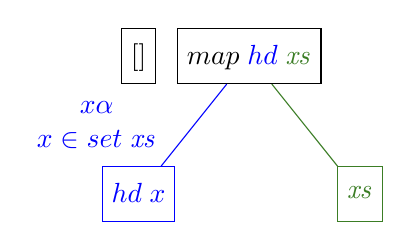
\begin{tikzpicture}
      \node [tree] (empty) {$[]$};
      \node [tree, right of=empty, node distance=4em] {$\holconst{map}\;\textcolor{Blue}{\holconst{hd}}\;\textcolor{OliveGreen}{\mathit{xs}}$}
        child [color=Blue] { node [tree] {$\holconst{hd}\;x$} edge from parent node [left, xshift=-1em, align=center] {$\holtypejudgement{x}{\alpha}$ \\ $x \in \holconst{set}\;\mathit{xs}$} }
        child [color=OliveGreen] { node [tree] {$\mathit{xs}$} };
    \end{tikzpicture}
    \caption{Forest with congruence rule for \holconst{map}}
    \label{fig:preproc:ctxtree:forest_with}
  \end{subfigure}
  \begin{subfigure}[b]{.53\linewidth}
    \small
    \[
      \inferrule*{
      }{\holconst{hd\_tl\_side}\;[]}
    \]
    \[
      \inferrule*{
        \holconst{map\_side}\;\holconst{hd}\;\mathit{xs}\\
        \forall x.\;x \in \holconst{set}\;\mathit{xs} \implies \holconst{hd\_side}\;x
      }{\holconst{hd\_tl\_side}\;(x \cons \mathit{xs})}
    \]
    \caption{Side condition with congruence rule for \holconst{map}}
    \label{fig:preproc:ctxtree:condition_with}
  \end{subfigure}
  \vspace{1em}

  \begin{subfigure}[b]{.45\linewidth}
    \centering
    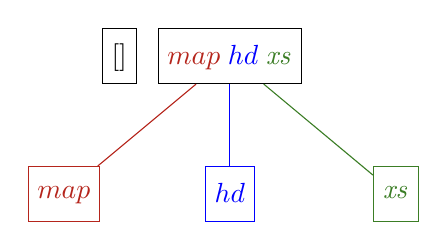
\begin{tikzpicture}[sibling distance=6em]
      \node [tree] (empty) {$[]$};
      \node [tree, right of=empty, node distance=4em] {$\textcolor{BrickRed}{\holconst{map}}\;\textcolor{Blue}{\holconst{hd}}\;\textcolor{OliveGreen}{\mathit{xs}}$}
        child [color=BrickRed] { node [tree] {$\holconst{map}$} }
        child [color=Blue] { node [tree] {$\holconst{hd}$} }
        child [color=OliveGreen] { node [tree] {$\mathit{xs}$} };
    \end{tikzpicture}
    \caption{Forest without congruence rule for \holconst{map}}
    \label{fig:preproc:ctxtree:forest_without}
  \end{subfigure}
  \begin{subfigure}[b]{.53\linewidth}
    \small
    \[
      \inferrule*{
      }{\holconst{hd\_tl\_side}\;[]}
    \]
    \[
      \inferrule*{
        \holconst{map\_side}\;\holconst{hd}\;\mathit{xs}\\
        \textcolor{Brown}{\forall x.}\;\holconst{hd\_side}\;\textcolor{Brown}{x}
      }{\holconst{hd\_tl\_side}\;(x \cons \mathit{xs})}
    \]
    \caption{Side condition without congruence rule for \holconst{map}}
    \label{fig:preproc:ctxtree:condition_without}
  \end{subfigure}

  \caption{Context forests and resulting side conditions of \holconst{hd\_tl}}
  \label{fig:preproc:ctxtree}
\end{figure}

\paragraph{Transformation to forest}
The routine starts by importing the (unstructured) set of congruence rules into a dedicated data structure (\cref{code:preproc:ctxtree}).
Then, the right-hand sides of all defining equations are converted into a \emph{context tree.}
Each node of the tree is labelled with a term and optionally, a congruence rule, and may have arbitrarily many children.
An edge from a node to a child is labelled with a \emph{context:}
a list of variables and of assumptions.

\remark*{
  In usual Isabelle parlance, a ``context'' would refer to a \texttt{Proof.context} that may contain arbitrary data; in this case, it is just fixed variables and assumptions.
}

\noindent
An example based on the $\holconst{hd\_tl}$ function is given in \cref{fig:preproc:ctxtree}.
It illustrates how the congruence rule of \holconst{map} participates in the transformation.

The transformation algorithm itself can be summarized as follows.
For a term $t$, a node is generated.
Then, it adds children to the node by case distinction on the shape of $t$:
\begin{itemize}
  \item
    If $t$ is atomic, it becomes a leaf node.
  \item
    If $t$ is a function application $\holconst{f}\;x_1\;\ldots\;x_n$, it tries to find a congruence rule that matches the term.
    $k$ children are added to the node according to the $k$ premises of the rule, tracking their variables and assumptions as context of the respective child.
    If there is no matching rule, the function and its arguments are considered separately, hence creating $n+1$ children.
  \item
    Otherwise, $t$ is an abstraction $\lambda x.\;u$.
    One child for $u$ is added with $x$ as context.
\end{itemize}

\noindent
In \cref{fig:preproc:ctxtree:forest_with}, there are two trees.
\begin{itemize}
  \item $\holconst{hd\_tl}\;[] = []$ gives rise to the tree with just a leaf node $[]$, because $[]$ is an atomic constant.
  \item $\holconst{hd\_tl}\;(x \cons \mathit{xs}) = \holconst{map}\;\holconst{hd}\;\mathit{xs}$ produces a node with two children, after applying the congruence rule for \holconst{map}.
    The left child has a context enriched with a variable and assumption, whereas the right child is the atomic $\mathit{xs}$.
\end{itemize}

\noindent
Ignoring the congruence rule results in the forest in \cref{fig:preproc:ctxtree:forest_without}, where three children are generated for the binary call to \holconst{map}.

\paragraph{Transformation to predicate}
Finally, the tree is transformed into a set of introduction rules for the inductive predicate representing the specifiedness.
\cref{fig:preproc:ctxtree:condition_with} illustrates the result of the transformation.
In a tree, each path from root to the side condition generates one assumption in the side condition based on the pre-existing side conditions, unless:
\begin{itemize}
  \item it is the first child of a function application with no matching congruence rule (nothing is known about that function call), or
  \item it is a free variable (always specified), or
  \item no side condition is known about the term (assumed total).
\end{itemize}

\noindent
Crucially, each layer of the tree still contributes to the side condition.
In the running example, this means that the root node contributes the assumption $\holconst{map\_side}\;\holconst{hd}\;\mathit{xs}$.

A special case arises in \cref{fig:preproc:ctxtree:condition_without}, where an assumption is generated for the node \holconst{hd}.
Because the forest has been created without a suitable congruence rule, there is no variable in the context of the node.
The transformation hence introduces a synthetic variable and universally quantifies over it (marked brown in the figure).
It can be proved that $\forall x.\;\holconst{hd\_side}\;x$ is false, because there is a list that violates $\holconst{hd\_side}$: the empty list.
In general, absence of congruence rules or congruence rules that are too weak may lead to vacuous side conditions.

The side condition for \holconst{undefined} is a prime example for being vacuous by definition:
there are no defining equations, hence no context trees, hence the inductive predicate is the empty least-fixed point.
The \holcommand{inductive} package admits such empty predicates.
They are logically vacuous, i.e., $\holconst{undefined\_side} \biimplies \holconst{False}$.

\paragraph{Simplification}
To avoid overly complicated side conditions, there are two strategies to simplify them.
The routine tries to:
\begin{enumerate}
  \item prove totality, i.e.\ $\forall x_1 \ldots x_n.\;\holconst{f\_side}\;x_1\;\ldots\;x_n$, and
  \item discharge auxiliary side conditions, e.g.\ $\holconst{hd\_side}\;(x \cons \mathit{xs}) = \holconst{True}$.
\end{enumerate}

\noindent
Both work by suitable preprocessing of the goal, then running Isabelle's full simplifier.
While this can make the result unpredictable, I have found that this prevents many redundant assumptions.

For the example in \cref{fig:preproc:ctxtree}, this removes the assumption $\holconst{map\_side}\;\holconst{hd}\;\mathit{xs}$, because $\holconst{map\_side}$ can be proved to be total.

\remark*{
  It is important to note that the generated side conditions are \emph{shallow}, that is, they only characterize the specifiedness of one function, but not any other non-constant functions, i.e.\ functions that are passed in as parameters, that are called along the way.
  This is nicely illustrated by this example:
  While the \holconst{map} function is obviously fully specified, it can be used in a partially specified way; namely, when the mapping function is only partially specified.
  The challenges to fully capture specifiedness are described in §\ref{sec:preproc:limitations}.
}

\subsubsection{Differences to Krauss' routine}

As indicated above, the \holcommand{function} package employs a similar routine.
The differences are mainly technical in nature, but are significant enough to prevent code reuse.
\begin{itemize}
  \item
    The internally produced congruence tree is not exported as a data structure.
  \item
    Traversal happens on an intermediate constant that represents all functions in a mutually recursive bundle with tupled arguments.
    For example, simultaneous recursive definitions of \holconst{odd} and \holconst{even} functions would internally be presented as a single function of type $(\holtype{nat} + \holtype{nat}) \Rightarrow (\holtype{bool} + \holtype{bool})$, where $\alpha + \beta$ denotes the sum type of $\alpha$ and $\beta$.
  \item
    Side conditions of auxiliary constants (in the running example: \holconst{map} and \holconst{hd}) are not considered: after defining and proving a function to be terminating, it is ``total'' by virtue of completion.
\end{itemize}

\noindent
Notably, the extraction of a termination relation -- just like specifiedness -- critically depends on the presence of appropriate congruence rules.
Similarly to the special case described above, absence of congruence rules may lead to unprovable termination relations.
Consequently, it is reasonable to assume that a user of the \holcommand{function} package is aware of this required setup; hence, it is not an extra burden to require the same setup for the dictionary construction.

\subsection{Correctness proofs}
\label{sec:preproc:dict:equiv}

There are two kinds of propositions that need to be proved in the routine:
dictionary certificates and equivalence theorems (§\ref{sec:preproc:dict:elim:encoding}).
In general, they are of the form:
\begin{align*}
  \ldots &\implies \holconst{cert\_}c\;(\holconst{inst\_}c\holconst{\_}\kappa\;\mathit{dict}_1\;\ldots) \\
  \ldots &\implies \holconst{f'}\;\mathit{dict_1}\;\ldots\;x_1\;\ldots = \holconst{f}\;x_1\;\ldots
\end{align*}
Both can carry preconditions for auxiliary dictionary certificates, and in the case of the equivalence theorems, also side conditions of the arguments $x_i$ (§\ref{sec:preproc:dict:partial}).
The proof strategies for both kinds of theorems differ, so I will discuss them separately.
Both strategies have in common that they require the proofs to happen in exactly the same (topological) order as the dictionary construction itself (\cref{fig:preproc:graph}).
At any point during a sequence of proofs, the previous correctness theorems are referred to as \emph{base theorems.}

\paragraph{Dictionary certificates}
Recall the definition of $\holconst{cert}\_c$ and $\dictinst{\holtypejudgement{\kappa}{c}}$.
The latter is a plain constructor application ($\holconst{mk}\_c$); the former inspects each field.
In other words, $\dictinst{\holtypejudgement{\kappa}{c}}$ ``bundles'' existing constants into a dictionary.
Consequently, the proof proceeds by simple application of the base theorems.

\paragraph{Equivalence theorems}
In general, these theorems need to be proved by induction using the induction scheme generated by the side condition, or if the side condition is trivial, the termination relation of the function.
Both are similar, so I focus on the latter.

Applying the induction principle creates one proof obligation per defining equation.%
Recall the \holconst{sum\_list} function from §\ref{sec:preproc:dict:termination}.
The proof obligations after induction are (dictionary certificates omitted):
\begin{align*}
  \holconst{sum\_list'}\;\mathit{d}_1\;\mathit{d}_2\;[] &= \holconst{sum\_list}\;[] \\
  \holconst{sum\_list'}\;\mathit{d}_1\;\mathit{d}_2\;\mathit{xs} = \holconst{sum\_list}\;\mathit{xs} \implies \holconst{sum\_list'}\;\mathit{d}_1\;\mathit{d}_2\;(x\cons\mathit{xs}) &= \holconst{sum\_list}\;(x\cons\mathit{xs})
\end{align*}
These can be discharged by first unfolding the defining equations of \holconst{sum\_list'} and \holconst{sum\_list}.
Then, base theorems and induction hypotheses are applied by walking the congruence tree.
Note that the base theorems include equivalences for class constants and the corresponding dictionary fields.

\remark*{
  The reality is a bit more complicated:
  one equation may create multiple defining equations, because the \holcommand{function} command disambiguates equations.
  For example, consider the definition $\holconst{single}\;[x] = \holconst{True}$ and $\holconst{single}\;\mathit{xs} = \holconst{False}$.
  The package instantiates the second equation ($\mathit{xs} = y\cons\mathit{ys}$ and $\mathit{xs} = []$) to avoid ambiguities.
}

\subsection{Related work}
\label{sec:preproc:dict:related}

\paragraph{Dictionary construction}
Type classes have been pioneered by the Haskell programming language~\cite{morris2013classes,wadler1989adhoc}.
There, a very similar construction to here is used, replacing classes by records and instances by functions~\cite{peternson1993typeclasses,augustsson1993overloading,chen1992parametric}.
Additional complications arise because Haskell admits cyclic dependencies between class instances~\cite{laemmel2005syb}, which are prohibited in Isabelle and hence pose no problem for this work.
A further simplification compared with Haskell is that Isabelle only features an ML-style simply typed polymorphic lambda calculus without constructor or multi-parameter classes.

Idris, a dependently typed functional language, generalizes the concept of type classes to classes that can be parametrized by any value.
In more recent versions of Idris, they are called \emph{interfaces}.
Still, the elaboration of expressions with class constraints and class and instance declarations is surprisingly similar to here~\cite{brady2013idris}.

In Scala, type classes are represented in an object-oriented style with objects and implicits~\cite{oliveira2010typeclasses}.
Type classes are just regular classes that are subject to the same compilation process to the Java Virtual Machine (and other backends).
Instances are also regular functions and constraints regular function arguments.
However, programmers do not need to pass instances manually; the compiler fills them in automatically.
The end result again is similar to that of Haskell and Idris, albeit it is mostly visible in the surface syntax instead of hidden in some intermediate compiler representation.

For Isabelle, Haftmann and Nipkow give a pen-and-paper correctness proof of the dictionary construction construction \cite[§4.1]{haftmann2010codegeneration}, based on a notion of \emph{higher-order rewrite systems}.
The resulting theorem states that any well-typed term is reduction-equivalent before and after class elimination.
In this work, the dictionary construction is performed in a certified fashion, that is, the equivalence is a theorem inside the logic.

\paragraph{Partially specified functions}
The notion of functions that are not defined universally for all possible (i.e.\ type-correct inputs) is pervasive in programming languages.
For example, major functional languages, like Haskell, Scala, and OCaml admit introduction of unspecified behaviour by allowing incomplete pattern matches.
The respective run-time environments throw an exception which can be caught by the caller of an underspecified function.
This is not generally how it works in total logics, where it is impossible to carry out non-trivial proofs about unspecified values.

However, much work on modelling partiality in proof assistants is centred around partiality induced by non-termination, instead of under-specification.
Finn \etal~\cite{finn1997partial} introduce an approach for the \emph{LAMBDA} system that tackles both issues in a similar way as Isabelle/HOL.
The undefined or arbitrary constant can be defined in terms of Hilbert's choice operator: under the assumption that $\tau$ is inhabited, $\epsilon \holtypejudgement{x}{\tau}.\;\holconst{False}$ delivers a value of type $\tau$ that is otherwise unspecified.
The authors use a similar example (head of a list) and point out that the usual axioms of classical logic still apply; for example, $\holconst{hd}\;[] = 5 \vee \holconst{hd}\;[] \neq 5$ is provable regardless of the unspecified result of retrieving the head of an empty list.
They also give a routine that, given a set of recursive equations, defines a domain predicate and a function that is qualified on that predicate.
My approach (§\ref{sec:preproc:dict:partial:spec}) is similar to the one by Finn \etal, with the notable improvement that I support higher-order recursion.

Cheng and Jones~\cite{cheng1991usability} give a survey of the treatment of partial functions, with the focus on usability.
They examine a total of eight different approaches:
restricting functions to a set while defining them,
treating functions as relations,
employing a different notion of equality,
extending logical operators to handle undefined values,
three-valued logics,
introducing a distinction between strict and total and non-strict and non-commutative connectives,
introducing a distinction between computation and reasoning, and finally,
adding a separate judgement for definedness.
My approach is most closely related to the last of these, which has initially been described by Plotkin as \emph{Partial Function Logic}~\cite[§9]{cheng1991usability}.
The notable difference is that the definedness judgement is represented as ``normal'' boolean predicates in the logics.
